\section{Data preprocessing}\label{sec:data-preprocessing}
To fulfill the requirements of the adapted transfer learning model the preprocessing tool was developed alongside a whole bunch of settings.
The collected data sequences are in form of coordinates' series, so it is necessary to represent them as 3-dimensional pictures which are the input to the convolutional neural network.
The described tool allows transferring those sequences into multidimensional arrays of numbers and also scale them to the required input size of a used transfer learning model.

\begin{figure}[!hbt]
    \center
    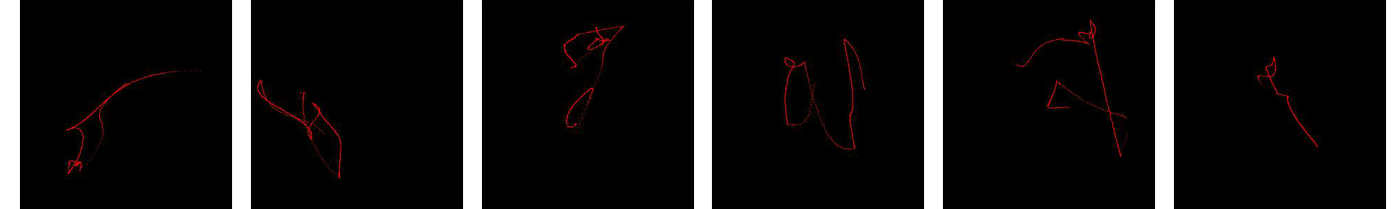
\includegraphics[width=\linewidth]{resources/bot_sequences}
    \captionof{figure}{Collected and preprocessed bot sequences with applied linear interpolation}
    \label{fig:bot_sequences}
\end{figure}
\begin{figure}[!hbt]
    \center
    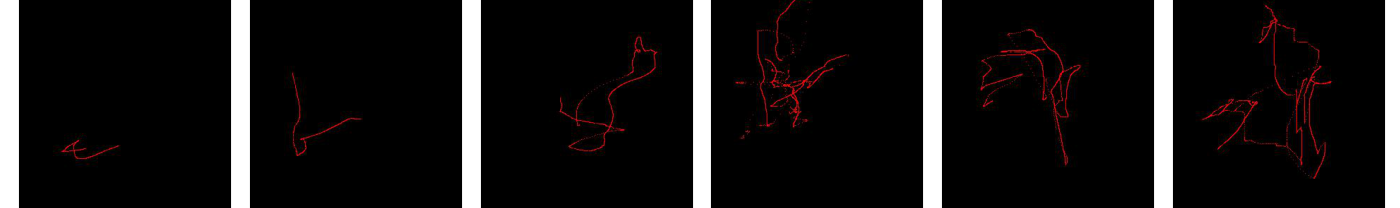
\includegraphics[width=\linewidth]{resources/user_sequences}
    \captionof{figure}{Collected and preprocessed user's sequences with applied linear interpolation}
    \label{fig:user_sequences}
\end{figure}


The data consists of isolated points that are result of discrete sampling, so to improve performance efficiency these points that represent the original coordinates on the user's screen are interpolated using a linear interpolation technique.
The operation was performed by connecting the discrete points using straight lines, so each consecutive event's coordinates were combined into a chain that results in a continuous curve on the input pictures.
The input data with applied linear interpolation and resizing are visualized in Fig.~\ref{fig:bot_sequences} and Fig.~\ref{fig:user_sequences}.
It was verified on the collected dataset that interpolated data results in better accuracy of a model in comparison to the isolated ones.
The presented tool works also as a splitter between training and testing sets using the provided ratio between them and as a label assigner which allows adding the corresponding labels to the single sequence basing on the provided identifier of the bot user.
Using this tool it is also possible to increase the number of bot samples by using several repetitions of the original bot set in cases of an imbalanced dataset.
The output of the preprocessor is a tuple of training and testing dataset along with labels, which can be directly the input of a neural network model.

In further work, in order to improve the performance of the model, data augmentation was introduced and applied.
A detailed description will be provided in Section~\ref{sec:machine-learning-model}, but it is worth mentioning that this approach required changes in the preprocessor tool.
The preprocessor was extend to allow saving interpolated and scaled images to the directory provided by the user.
Along with the extensions in the preprocessor, the main script was enhanced with the ability to load the dataset from image files.
The previous option --- loading from binary files --- was unchanged.